%% Common template of the research article using elsarticle class.
%% The elsarticle class provided by Elseiver (see http://www.elsevier.com/author-schemas/latex-instructions).
%% 
%% Author: Dmitriy O. Afanasyev
%% Email: dmafanasyev@gmail.com
%% Web: http://dmafanasyev.ru
%% Version: 1.0, Feb 04, 2015
%% 
%% ---------------------------------------------
%% 
%% It may be distributed under the conditions of the LaTeX Project Public
%% License, either version 1.2 of this license or (at your option) any
%% later version.  The latest version of this license is in
%%    http://www.latex-project.org/lppl.txt
%% and version 1.2 or later is part of all distributions of LaTeX
%% version 1999/12/01 or later.
%%

\documentclass[3p,11pt,authoryear]{elsarticle}
\usepackage[T1]{fontenc}
\usepackage[utf8]{inputenc}
\usepackage[english]{babel}
\usepackage{epstopdf,cmap,amssymb,amsfonts,amsmath,mathtext,
            enumerate,float,natbib,indentfirst,hyperref,
            graphicx,multirow,color,setspace,wrapfig}
% lmodern used for good quality english font rendering.
\usepackage{lmodern}

\graphicspath{{figures/}}

\journal{Journal Title}

\begin{document}

\begin{frontmatter}

%% title, authors, affilations
%% title
\title{Fine-grained mommagraphy object 
detection with multiple feature fusion 
transfer learning}

%% authors & affiliations
\author[add1,add2]{Ri-Gui Zhou}
\ead{rgzhou@shmtu.edu.cn}

\author[add1,add2]{Shihao Lv\corref{corrauthor}}
\ead{lvshihao@stu.shmtu.edu.cn}
\cortext[corrauthor]{Ri-Gui Zhou, Shihao Lv, 
Yaochong Li,
are with the College of Information 
Engineering, Shanghai Maritime University, 
Shanghai 201306, China and the Research 
Center of Intelligent Information Processing 
and Quantum Intelligent Computing, Shanghai 
201306, China.}


\author[add1,add2]{Yaochong Li}
\ead{liyaochong123@gmail.com}

\address[add1]{College of Information 
Engineering, Shanghai Maritime University, 
Shanghai 201306, China}
\address[add2]{Research Center of 
Intelligent Information Processing and 
Quantum Intelligent Computing, Shanghai 
201306, China}

%% abstract
\begin{abstract}
Breast cancer is the second leading cause of 
cancer deaths among women and screening 
mammography has been found to reduce 
mortality. It is necessary to build 
mammography image recognition systems. 
Previous solutions for mammography image 
recognition are usually based on hand-crafted 
features methods and use but limited in 
specific situations. Also, some methods 
utilize simple deep learning network, which 
can not extract the full feature of mammography,
for example, GoogleNet, VGG16, ResNet, DenseNet, etc.
In this paper, we propose a deep learning based 
approach with multiple feature fusion transfer 
learning strategy. Firstly, we obtain the 
training data from an open data set called 
DDSM images. Then we employ data augment 
methods, and training a deep convolutional 
neural network to extract image features and 
conduct the object detection job. 
A pre-trained model is used to initialize the 
network and help extract the basic features.
Furthermore, we propose a fusion method that 
makes use of multiple transfer learning models 
in inference, to improve the accuracy on the 
test set. Importantly, we take a strategy 
applied by hash learning in the deep network 
is cited to enhance the generalization ability 
of the model and solve the challenge of 
high-dimensional calculation in deep learning. 
In the end, regression analysis to analyze 
the object position. The experimental results 
prove that our method achieves high accuracy on 
the mammography image object detection 
and inspection task.
\end{abstract}

%% keywords
\begin{keyword}
CNNs \sep Random Forest \sep Learning to Hash  \sep DensNet \sep Feature Fusion
\end{keyword}

\end{frontmatter}

%% main text
\section{Introduction}
\label{sec:Intro}

The rapid development of machine learning and 
especially deep learning has attracted the medical 
imaging community’s interest in applying these 
techniques to improve the accuracy of cancer 
screening. Breast cancer is the second leading 
cause of cancer deaths among U.S. women and 
screening mammography has been proved to reduce 
mortality
\cite{Oeffinger2015,Zhu2019}.
According to a study by the Breast 
Cancer Surveillance Consortium in 2009, the 
overall sensitivity of digital screening mammography 
in the U.S. is 84.4$\%$ and the overall specificity 
is 90.8$\%$
\cite{Jamieson2012}.
To help radiologists improve 
the predictive accuracy of screening mammography, 
computer-assisted detection and diagnosis (CAD) 
software have been developed and in clinical 
diagnosis since the 1990s. Unfortunately, data 
suggests that commercial CAD systems have not led 
to significant improvement in performance and 
progress has stagnated in the past decade
\cite{Girshick2015}.
With the remarkable success of deep learning in 
visual object recognition and detection, and many 
other domains have paid more attention to it
\cite{Lecun2015}.
There is much interest in developing deep 
learning tools to assist radiologists and improve 
the accuracy of screening mammography. 

Early detection of subclinical breast cancer on 
screening mammography is challenging as an image
classification task because the tumors themselves 
occupy only a small portion of the image of the
entire breast. For example, a full-field digital 
mammography (FFDM) image is typically 4000 × 3000
pixels while a cancerous region of interest (ROI) 
can be as small as 100 × 100 pixels. If ROI
annotations were widely available in mammography 
databases then established object detection and
classification methods such as the region-based 
convolutional neural network (R-CNN) and its
variants could be readily applied
\cite{Girshick2014,Girshick2015,Ren2017}.
However, approaches that require ROI annotations 
\cite{Dai2016}
often cannot be transferred to large mammography 
databases that lack ROI annotations, which are
laborious and costly to assemble. Indeed, few 
public mammography databases are annotated.
Yet, deep learning requires large training datasets 
to be most effective. Thus, it is essential to 
leverage both the few fully annotated datasets, as 
well as larger datasets labeled with only the 
cancer status of each image to improve the accuracy 
of breast cancer classification algorithms.

Pre-training is a promising method to address the 
training problem. For example 
\cite{Hinton2006,Li_2020},
used layer-wise pre-training to initialize the 
weight parameters of a deep belief net (DBN) with 
three hidden layers and then fine-tuned it for 
classification. They found that pre-training 
improved the training speed as well as the 
accuracy of handwritten digit recognition. Another 
popular training method is to first train a deep 
learning model on a large database such as the 
ImageNet 
\cite{Russakovsky2015,9112355}
and then fine-tune the model for another task. 
Although the specific task may not be related to 
the initial training dataset, the model’s weight 
parameters are already initialized for recognizing 
primitive features, such as edges, corners and 
textures, which can be readily used for a different 
task. This often saves training time and improves 
the model’s performance
\cite{He2016,Moreira2018}.

To take advantage of feature extraction ability of 
CNNs, recently researchers have proposed new 
mammography recognition methods. However, we think 
the ability to extratct the image features of 
deep CNNs could be better utilized. In this study, fusing 
different deep neural network models together to 
propose a fine-grained mammography image 
recognition approach via fusing multiple learned
features. Besides, utilizing the hash decoder
method to simplifying the classification 
calculation of complex high-dimensional 
feature vectors, and fusing the results of 
different classifier in the end. Our work can 
be summarized as follows:

1. Build a deep convolutional neural network based 
on well-performed network structures, and design a 
transfer learning strategy to improve the 
representation power of the extracted features.


2. To further utilize the feature representation 
ability of CNNs, we propose a method to fuse 
extracted features from multiple trained models 
with similar topological structure to
further improve the classification accuracy.

3. The strategy applied by hash learning in the 
deep network is cited to enhance the 
generalization ability of the model and solve the 
challenge of high-dimensional calculation 
in deep learning.

4. The designed feature fusion model is used in 
the feature extraction process of Faster RCNN, 
and a deep hash learning strategy is introduced 
in the classification stage.

The rest of this paper is organized as follows. 
Section~\ref{sec:Meth} 
details of the network structure and the proposed 
method. 
Section~\ref{sec:Data} 
elaborates the dataset used in our work.
Section~\ref{sec:Exp} 
demonstrates the experiment results and gives 
discussion. 
Section~\ref{sec:Conc} 
makes the conclusion and future work are provided 
in the end.

\begin{figure*}[!ht]
    \centering
    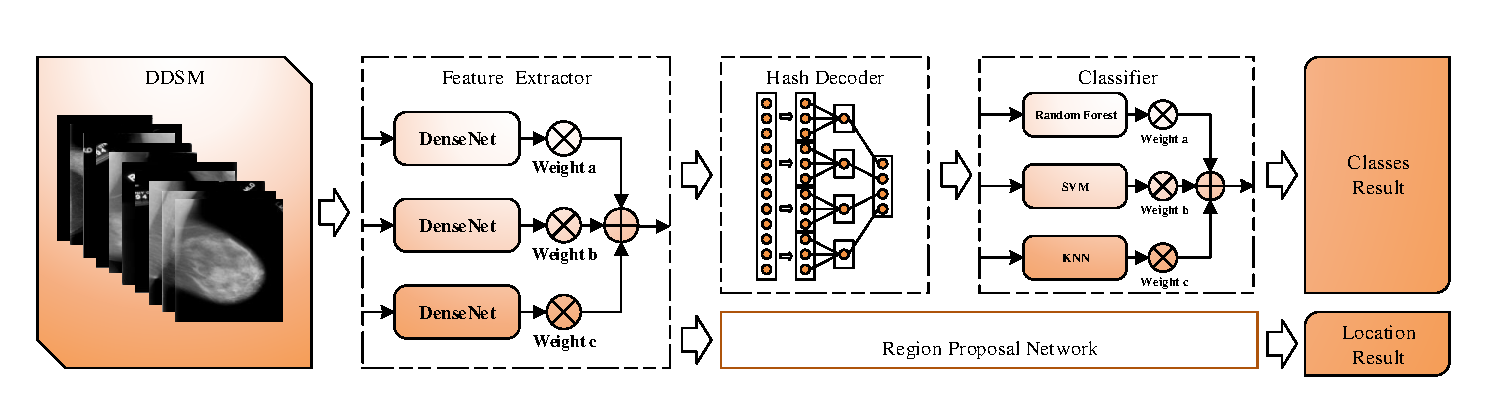
\includegraphics[
        width=1.0\textwidth,
        keepaspectratio
    ]{NetStruct.pdf}
    \caption{Overview of the proposed approach.}
    \label{fig:netStruct}
\end{figure*}


\section{Methodology}
\label{sec:Meth}

The architecture of our approach can be 
divided into 4 modules, as shown in 
Figure~\ref{fig:netStruct}. 
The first module is image feature extractor, which
contains three pretrained models of DenseNet, which 
are trained on ImageNet task is used as the 
backbone of our network structure. Benefited from 
pre-trained models, the network gains the ability to 
extract basic features from images before training. 
Designing three different models has aimed for 
diverse features. To make use of different 
representation power of each model, fusing the
feature from each model with weight add method.
The second module is a hash decoder, which is aim
at dividing randomly image features into multiple 
branches, with each branch corresponding to one 
hash bit. Through such steps, the model can not 
only improve the generalization ability of the 
model, but also simplify the calculation of 
high-dimensional features to facilitate the work 
of the classifier.
The third module is employed to perform 
classification, we also has 
used three classifiers which contains SVM(Support
Vector Machine), KNN(K Nearest Neighbor) and 
RF(Random Forest). This design of classifications 
is to help improve the accuracy of model 
predictions.
The fourth module is a linear regression analysis 
model, which utilied the RPN(Region Proposal 
Network) proposed by Faster RCNN. To do this, 
it is aimed at marking the specific location of the 
lesion in mammography.

\subsection{Network design}
\label{sec:MethNet}

Hand-crafted features have been widely used in the
image classification tasks, including mammography 
image classification tasks. Though these 
hand-crafted feature based methods perform well, 
they are always too complicated to build and could 
be constrained in specific situations. With the 
development of deep learning techniques, deep 
convolutional neural networks have achieved 
great success in image analysis task, because of 
its ability to extract intricate features from 
raw data
\cite{Szegedy2016,Zeiler2014}.
By training a model with a huge amount of images, 
the learned parameters network could gain greater 
representation power and perform better than 
hand-crafted feature based methods
\cite{Jamieson2012}.
Hence we decide to build a mammography images 
object detection network. CNNs based approaches 
on mammography image 
recognition tasks have been proposed in recent 
years, most of them train a single neural network 
model to extract image features
\cite{He2019}.
After AlexNet achieved great success in the 
ImageNet competition, the potential of deep CNNs 
are gradually discovered by researchers, many deep 
network architectures with good performance on 
image classification tasks such as VGGNet, 
GoogLeNet, ResNet, DenseNet and etc, network 
based on these well-performed architectures are 
naturally applied to mammography image recognition 
task. We build a fusion network made of four 
modules which are feature extractor(Explained 
in detail in 
Section~\ref{sec:MethNetFea}), 
hash decoder(Explained in detail in 
Section~\ref{sec:MethNetHash}),
classifier(Explained in detail in 
Section~\ref{sec:MethNetCls}) 
and regression model(Explained in detail in 
Section~\ref{sec:MethNetReg}). 

\subsubsection{Feature Extract Module}
\label{sec:MethNetFea}

In the feature extractor modules, building it 
with a truncated DenseNet without the fully 
connected layers. The backbone of DenseNet
consists of 3 dense blocks, each dense block 
is composed of several dense layers. The 
number of dense layers in each dense block 
increases while the dense blocks go deeper.
The structure of a dense block is shown in 
Figure~\ref{fig:DenseBlock}.

\begin{figure*}[!ht]
    \centering
    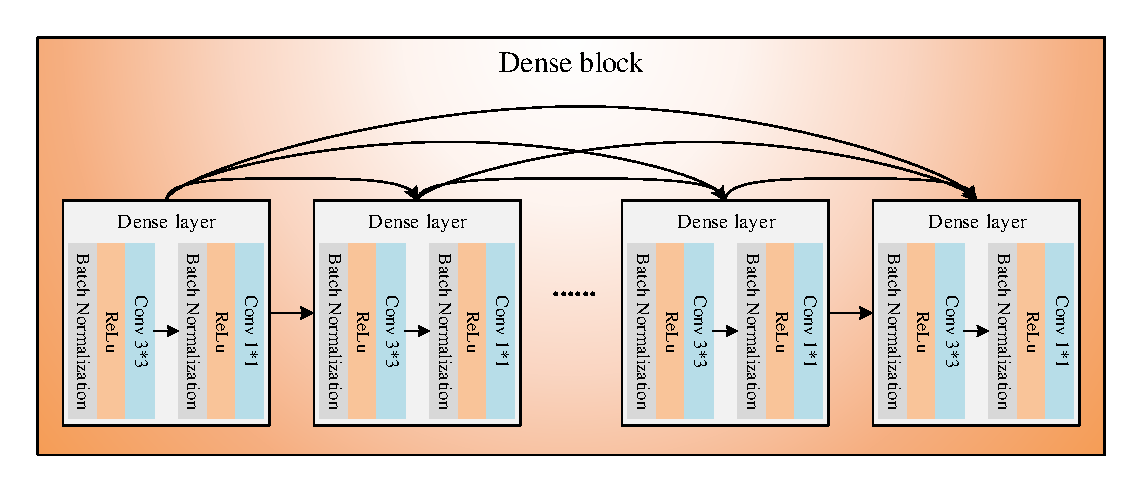
\includegraphics[
        width=0.78\textwidth,
        keepaspectratio
    ]{DenseBlock.pdf}
    \caption{The architecture of DenseNet.}
    \label{fig:DenseBlock}
\end{figure*} 

As for the DenseNet, different from a normal 
convolutional neural network, each dense 
layer’s output is fed to all subsequent dense 
layers in the same block through the dense 
connections, which is implemented by 
concatenation operations. In this way, global 
information can traverse the dense block from 
beginning to end, each dense layer can 
acquire extra knowledge from the previous ones. 
For a dense layer, it includes 2 basic layers, 
each basic layer is composed of a batch 
normalization layer, a ReLU activation 
function
\cite{Srivastava2014,Ioffe2015,Kingma2015} 
and 2 convolutional layers. The first 
convolutional layer with a 1 × 1 kernel is 
called the bottleneck layer, and it helps to 
reduce the feature map dimension to improve 
calculation efficiency. The second layer 
applies a 3 × 3 kernel to extract features. 
Benefit from densely connections, the network 
can extract more representative features than 
the normal convolutional network with layers 
connected in sequence. In addition, an 
attention block and a transition block are 
inserted between every two dense blocks. The 
attention block helps the feature extractors 
locate the most informative part of the 
input feature map. The transition block 
consists of a batch normalization layer 
and a 1 × 1 convolutional layer followed 
by 2 × 2 max pooling layer. It is set for 
down sampling the output feature maps of 
each dense block. While network goes deeper, 
the size of output feature maps decreases 
and the dimension of output feature maps 
increases. An example of the output feature 
maps after each dense block is shown in 
Figure~\ref{fig:imgFea}.

\begin{figure*}[!ht]
    \centering
    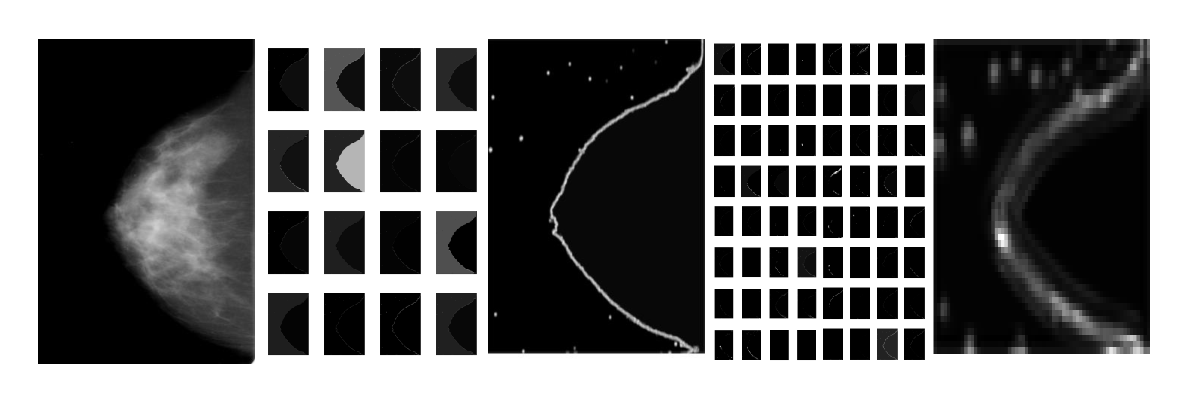
\includegraphics[
        width=1.0\textwidth,
        keepaspectratio
    ]{ImgFea.pdf}
    \caption{The feature of the 
        fusion of extractors' result.}
    \label{fig:imgFea}
\end{figure*} 

Usually, most CNN based methods on mammography 
image classification tasks use a single network 
to extract features, and then feed them into 
a classifier. However, we found that AGNet
did this job in a different way. It tried to 
explore the potential power of fusion features 
extracted from different models. In which, two 
models are fused to predict the label of input 
image together, one is based on AlexNet and  
there is based on GoogLeNet. It takes 
advantage of different features with higher 
accuracy than the single network methods.
Inspired by AGNet, proposing an approach to 
improve the classification accuracy by 
fusing multiple models with the same structure 
trained with different transfer learning 
strategies. Note that shallower layers tend to 
extract basic features, deeper layers tend to 
extract abstract feature, concluding that 
models with different layers’ parameters 
fixed during the training phase would focus on 
features with different complexity.
\cite{Ciresan2012}
At the inference phase, we fuse the trained models 
together to make use of the different 
feature extraction ability of each model.

Different from AGNet, train 3 models with 
the same structure, but freeze different 
layers of each model while training 
concurrently. There are two reasons why we 
select 3 same DenseNet based model to be fused. 
Firstly, we have tested the single-model 
method for this task, among which DenseNet
performs best. Secondly, we have tried fusing 
different trained models such as Inception, 
ResNet, DenseNet structures together with frozen 
parameters, fusing 3 DenseNet based models 
is still the better way. We think the reason 
is that when fusing models in different 
topological structures, the relationship 
between features extracted from 3 models is 
relatively weak and we cannot assure that 
they are learning different knowledge from 
training images. Since the structures of 
different networks varies greatly, models may
concentrate on similar features with different 
performance according to the depth of network. 
By training 4 similar structure models with 
different frozen layers, each model extracts 
features in different levels based on the 
number of frozen parameters, we can ensure 
that every model concentrates on different 
features of the input image. Meanwhile, in
the experiment we found the false positive 
and false negative instances of each model 
are quite different, which proves that they 
are concentrating on different kinds of 
features. Since the 4 models keep a similar 
network structure, the relationship between 
features they extracted are stronger,
and features can be fused better.

\begin{figure*}[!ht]
    \centering
    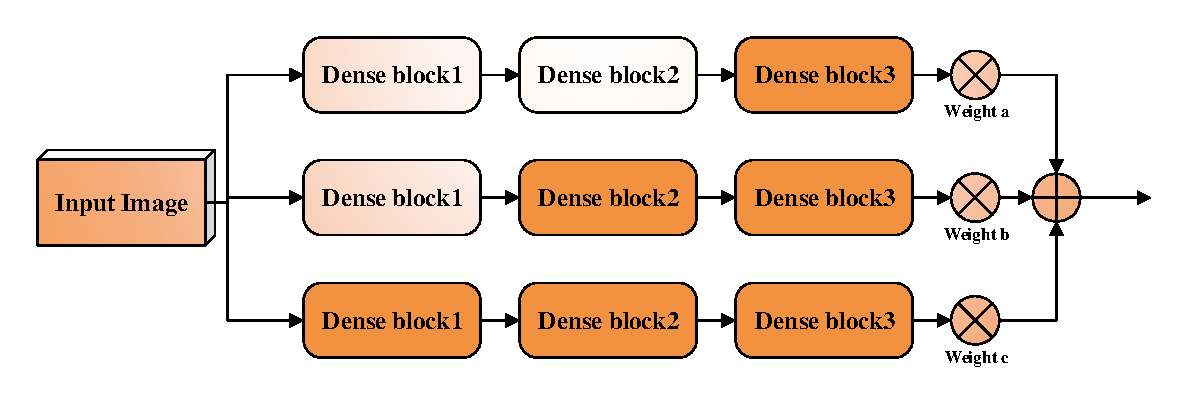
\includegraphics[
        width=0.78\textwidth,
        keepaspectratio
    ]{ExtractorFusion.pdf}
    \caption{The module of feature extractors' 
        fusion.}
    \label{fig:extrFusion}
\end{figure*} 

As figure~\ref{fig:extrFusion}
shows, training 3 models with parameters in 
different block frozen in parallel. Each row 
represents one model, the dense block in 
bright means that the parameters in this 
block are frozen during the training phase 
while the dark block means that parameters 
are activated. we fuse the feature of multiple 
transfer learning models with a weighted
sum operation. The weights of 3 models are 
set manually in the experiments. Taking the 
advantage of features diversity, the transfer 
learning models fusion method achieved high
accuracy in the mammography image recognition
task. 


\subsubsection{Hash Decoder Module}
\label{sec:MethNetHash}

After obtaining intermediate image features 
from the module of feature extractor, we
propose a hash decoder module to map these 
image features to hash codes. 
We assume each target hash code has q bits. 
Then the outputs of the feature extractor 
are designed to be 50q. As can be seen in 
Figure~\ref{fig:hashDecoder}, 
the proposed hash decoder module firstly 
divides randomly the features vectors into 
q slices with equal length 4. Then each 
slice is mapped to one dimension by a 
fully-connected layer, followed by a 
sigmoid activation function that restricts 
the output value in the range [0, 1],
and a piece-wise threshold function to 
encourage the output of binary hash bits. 
After that, the q output hash bits are
concatenated to be a q-bit code. A possible 
alternative to the hash decoder module is 
a simple fully-connected layer that maps 
the input intermediate image features into 
q-dimensional vectors, followed by sigmoid 
activation functions to transform these 
vectors into [0, 1]. Compared to this 
alternative, the key idea of the overall 
strategy is trying to reduce the redundancy 
among the hash bits. Hash codes with fewer 
redundant bits are advocated by some recent 
research. 

\begin{figure*}[!ht]
    \centering
    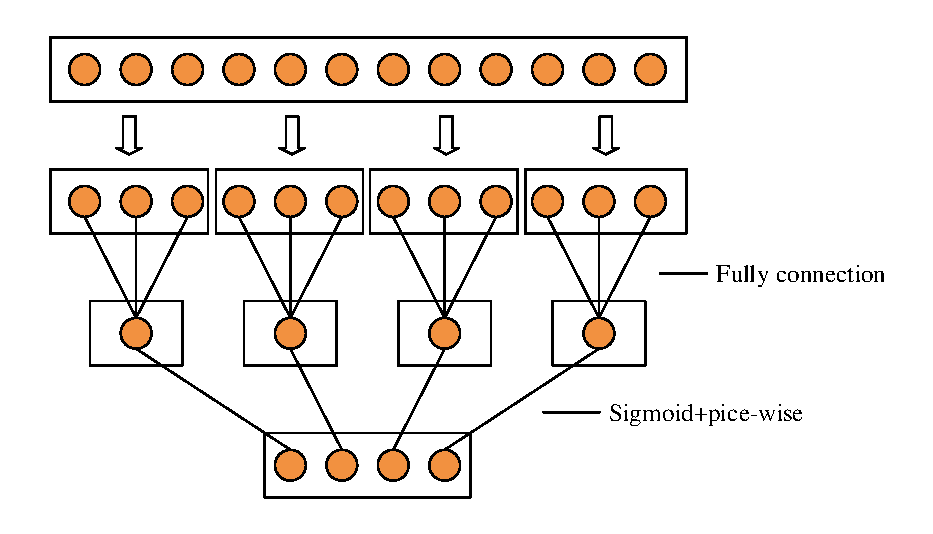
\includegraphics[
        width=0.66\textwidth,
        keepaspectratio
    ]{HashDecode.pdf}
    \caption{The module of the hash decoder.}
    \label{fig:hashDecoder}
\end{figure*} 

In order to encourage the output of a hash 
decoder to be binary codes, we use a sigmoid 
activation function followed by a piece-wise 
threshold function.
Given a 50-dimensional slice 
$x^{(i)}(i=1,2,...q)$
, the output of the 50-to-1 fully-connected 
layer is defined by

\begin{equation}
    \label{eq:eq_descr_1}
    fc_i(x^{(i)}) = W_ix^{(i)}
\end{equation}

with $W_i$ being the weight matrix.

Given $c=fc_i(x^{(i)})$, the sigmoid function
is defined by 

\begin{equation}
    \label{eq:eq_descr_2}
    sigmoid(c) = \frac{1}{1+e^{-\beta c}}
\end{equation}

where $\beta$ is a hyper-parameter.

The piece-wise threshold function is to 
encourage binary outputs. Specifically, for an 
input variable $s = sigmoid(c) \in [0,1]$, 
this piece-wise function is defined by

\begin{equation}
    \label{eq:eq_descr_3}
    y = \left\{
        \begin{array}{lr}
            0, & s < 0.5-\epsilon \\
            s, & 0.5-\epsilon \le 0.5+\epsilon \\
            1, & s > 0.5+\epsilon
        \end{array}
    \right.\nonumber,
\end{equation}

where $\epsilon$ is a small positive 
hyper-parameter.

This piece-wise threshold function 
approximates the behavior of hard-coding, 
and it encourages binary outputs in training. 
Specifically, if the outputs from the sigmoid 
function are in $[0, 0.5-\epsilon]$ or 
$[0.5+\epsilon, 1]$, they are truncated to be 
0 or 1, respectively. Note that in prediction, 
the proposed deep architecture only generates 
approximate (real-value) hash codes for input 
images, where these approximate codes are 
converted to binary codes by quantization. 
With the proposed piece-wise threshold 
function, some of the values in the 
approximate hash codes are already zeros or 
ones. Hence, less errors may be introduced
by the quantization step.

\subsubsection{Classifier Module}
\label{sec:MethNetCls}

In the classifier module, building it with
a fusion structure by SVM, KNN, Random
Forest classic methods. For each method, it 
predicates with the output of the hash decoder,
then the three results weight add, as the 
result of class information. There is a reason
why we select 3 different classifiers to be 
fused. These three algorithms target 
different classification types, so the 
results obtained for different feature 
information will also be different. The 
biggest advantage of doing this is to 
improve the robustness of the model, 
and at the same time it also improves 
the accuracy of model recognition. 

\begin{figure*}[!ht]
    \centering
    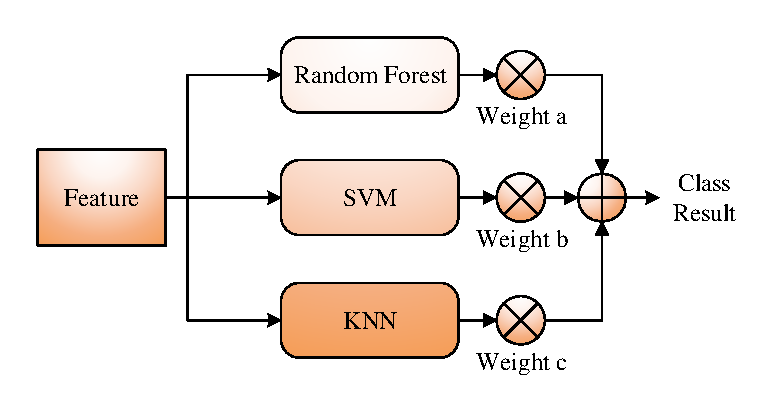
\includegraphics[
        width=0.58\textwidth,
        keepaspectratio
    ]{ClassifierFusion.pdf}
    \caption{The module of the fusion of 
        classifier.}
    \label{fig:classifierFusion}
\end{figure*}   

As for the KNN, which is simple, easy to 
understand, easy to implement, no need 
to estimate parameters, no training. 
As for the SVM,  after the training is 
completed, most of the training samples 
do not need to be retained, and the final 
model is only related to the support vector.
As for the Random Forest, which is based on 
an ensemble of decision trees where each of the 
trees is based on the randomly selected subset of 
the training set. Random forest uses slightly 
different kinds of bagging approach where a 
subset of features is selected for the split
at node, whereas in bagging all features are 
used for node split. As a result, the random 
forest is an aggregation of trees, which reduces 
the effect of noise present in a single tree.
Hence, bagging generally increases the 
overall result.

\subsubsection{Regression module}
\label{sec:MethNetReg}

A Region Proposal Network (RPN) takes an 
image (of any size) as input and outputs a 
set of rectangular object proposals, 
each with an objectness score. To generate 
region proposals, sliding a small network 
over the conv feature map output by the last
shared conv layer. This network is 
fully connected to an n × n spatial window 
of the input conv feature map. Each sliding 
window is mapped to a lower-dimensional vector. 
This vector is fed into two sibling 
fully-connected layers — a box-regression layer 
and a box-classification layer. As shown in
Figure~\ref{fig:RPN}

\begin{figure*}[!ht]
    \centering
    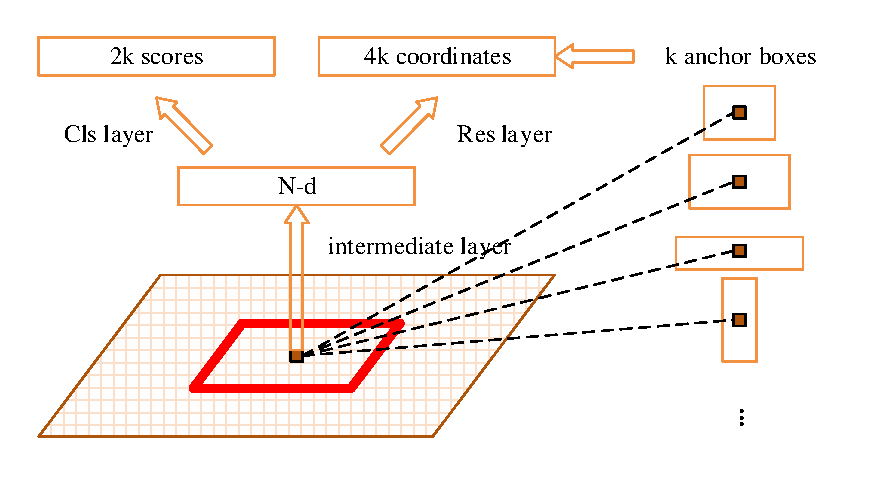
\includegraphics[
        width=0.68\textwidth,
        keepaspectratio
    ]{RPN.pdf}
    \caption{The module of the region proposal 
        network.}
    \label{fig:RPN}
\end{figure*} 


Note that because the mini-network operates
in a sliding-window fashion, the 
fully-connected layers are shared across 
all spatial locations. This architecture is 
naturally implemented with an n × n conv layer 
followed by two sibling 1 × 1 conv
layers. And the loss function is defined by

\begin{equation}
    \label{eq:eq_descr_4}
    L({p_i},{t_i})=\frac{1}{N_{cls}}\sum_iL_{cls}(p_i,p_i^*)
     + \lambda\frac{1}{N_{reg}}\sum_ip_i^*L_{reg}(t_i,t_i^*)
\end{equation}

Here, $i$ is the index of an anchor in a 
mini-batch and $p_i$ is the predicted 
probability of anchor $i$ being an object. 
The ground-truth label $p_i^*$ is 1 if the 
anchor is positive, and is 0 if the anchor 
is negative. $t_i$ is a vector representing 
the 4 parameterized coordinates of the 
predicted bounding box, and $t_i^*$ is that
of the ground-truth box associated with a 
positive anchor. The classification loss 
$L_{cls}$ is log loss over two classes 
(object $vs$ not object). For the regression 
loss, we use 
$L_{reg}(t_i, t_i^*)=R(t_i, t_i^*)$ where $R$
is the robust loss function (smooth $L_i$). 
The term $p_i^*L_{reg}$ means the regression 
loss is activated only for positive anchors 
and is disabled otherwise. The outputs of
the $cls$ and $reg$ layers consist of ${p_i}$ 
and ${t_i}$ respectively. The two terms are 
normalized with $N_{cls}$ and $N_{reg}$, and 
a balancing weight $\lambda$.

For regression, we adopt the parameterizations 
of the 4 coordinates following:

\begin{eqnarray}\label{eq:eq_descr_5}
    t_x=(x-x_a)/w_a, 
    t_y=(y-y_a)/h_a, 
    t_w=log(w/w_a), 
    t_h=log(h/h_a), \\
    t_x^*=(x^*-x^*_a)/w_a, 
    t_y^*=(y^*-y^*_a)/h_a, 
    t_w^*=log(w^*/w_a), 
    t_h^*=log(h^*/h_a)
\end{eqnarray}

where $x$, $y$, $w$, and $h$ denote the two 
coordinates of the box center, width, and 
height. Variables $x$, $x_a$, and $x^*$ are 
for the predicted box, anchor box, and 
ground-truth box respectively (likewise for 
$y$, $w$, $h$). This can be thought of as 
bounding-box regression from an anchor box 
to a nearby ground-truth box.

\subsection{Transfer learning}
\label{sec:MethTL}

Transfer learning aims to transfer knowledge 
between related source and target domains
\cite{Pan2010}.
It is a useful tool in machine learning, 
leading to a positive effect on the domains 
that are difficult to apply because of 
insufficient training data. Transfer learning 
methods can be categorized into 4 classes: 
instance-based, mapping-based, network-based,
adversarial-based deep transfer learning
\cite{Tan2018}.
Network-based method is mostly used in 
convolutional neural networks. It is achieved 
by transferring the network structure and 
pre-trained parameters of the source domain into 
a part of a deep convolutional neural network 
used in the target domain. In our work, 
we construct feature extractor as 
described in Section~\ref{sec:MethNetFea}, 
then we initialize the network parameters 
with the parameters of a DenseNet model 
that were pre-trained on the ImageNet dataset.

In our experiments, an input image is 
resized to a tensor, going that dataset; 
freezing, which consists of leaving the 
parameters in shallow part of the 
pretrained model unchanged and training 
only the rest part of the network, which can 
make use of the basic feature extracting 
ability of pretrained model. Freezing layers 
or not in training phase depends on the 
number of category and quantity variance 
between source and target dataset. 
Compared to ImageNet dataset, the DDSM 
dataset we used are much smaller. 
Moreover, most images in both datasets 
are natural images, they are similar in 
a way, hence we freeze some of the layers 
during training. In order to explore the 
effect of fusing different feature extractors, 
we try different freezing strategy on the 
networks, the details are described in 
Section~\ref{sec:MethNetFea}. 


\section{Data}
\label{sec:Data}

\subsection{DDSM}
\label{subsec: Date_DDSM}

Most computer-aided diagnosis (CADx) and 
detection (CADe) algorithms for breast cancer 
in mammography are evaluated on private data 
sets or on unspecified subsets of public 
databases. 
\cite{Gao2019}
This causes an inability to 
directly compare the performance of methods or 
to replicate prior results. 
\cite{Choukroun2017}
To resolve this substantial challenge by releasing 
an updated and standardized version of the 
Digital Database for Screening Mammography 
(DDSM) for evaluation of future CADx and CADe 
systems (sometimes referred to generally as CAD) 
research in mammography.
\cite{Zhu2017}
The CBIS-DDSM (Curated Breast Imaging Subset of 
DDSM), includes decompressed images, data 
selection, curation by trained mammographers, 
updated mass segmentation, bounding 
boxes, and pathologic diagnosis for training 
data, formatted similarly to modern computer 
vision data sets. The data set contains 753 
calcification cases and 891 mass cases, 
providing a data-set size capable of 
analyzing decision support systems in 
mammography. As shown in Figure~\ref{fig:figData}

\begin{figure*}[!ht]
    \centering
    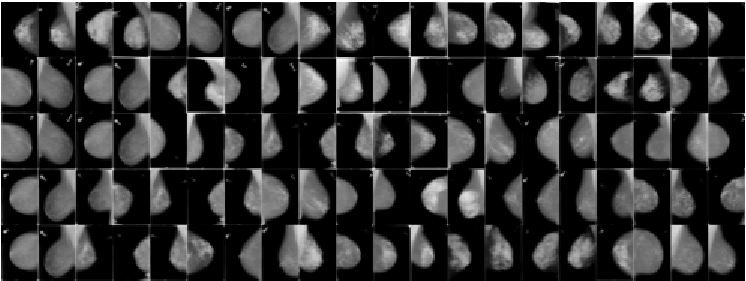
\includegraphics[
        width=1.0\textwidth,
        keepaspectratio
        ]{Data.pdf}
    \caption{Examples in the dataset}
    \label{fig:figData}
\end{figure*}

\subsection{Augmentation}
\label{subsec: Date_Aug}

Compared to other common data sets 
(e.g. Pascal Voc) in the field of image 
object detection, the DDSM data set 
is relatively small. 
\cite{M.HeathK.BowyerD.Kopans2001}
Since small data 
sets are prone to reduce the model effect, 
to maintain the representation power of 
model and avoid overfitting in some ways, 
several data augmentation methods are 
employed. We don’t augment data with the
crop, translate or scale operations to 
avoid changing the original label of images.
Instead, we randomly rotate and shear the 
original images between -10$^{\circ}$ and 
10$^{\circ}$ , then flip them horizontally 
or vertically and fill the margin with 
white pixels. 

\section{Experiments}
\label{sec:Exp}

\subsection{Training strategies}
\label{sec:ExpStra}

The approach of this study is implemented by 
the open source framework PyTorch. 
\cite{Abadi2016}
The pre-trained models for initializing the 
network parameters are acquired from 
torchvision.
\cite{Paszke2017}
Models are trained and tested on a graphic 
workstation with an Intel Core i9-7980XE 
CPU(2.60 GHz, 18 core) and a GeForce GTX 
1080Ti GPU. As described in 
Section~\ref{sec:Data}, 
we choose a dataset DDSM to train and test 
our proposed network in the experiments. 

In the training phase, we use a stochastic 
gradient descent method with a batch size of 32, 
\cite{Ioffe2015}
a momentum of 0.9 and a weight decay of 
0.0005 similar to optimize our models 
for 100 epochs. As shown in 
Figure~\ref{fig:extrFusion}, 
we propose a method fusing 3 models with 
similar structure and freezing different 
layers called Freeze1 to Freeze3 from top to 
bottom. The accuracy curves on the 
validation dataset of 3 models in the 
training phase are shown in 
Figure~\ref{fig:resAcc}. 
Due to the warmup strategy,
\cite{Glorot2011}
the accuracy grows 
slowly in the first 5 epochs. A relatively 
large batch size reduces the noise in the 
gradient, and an increased learning rate 
can make a larger progress along the 
opposite of the gradient direction.
\cite{Liu2020}
Since our network structure is based on 
DenseNet, the learning rate is initialized to 
0.01 and lowered by 10 times every 20 
epochs in the experiments.
\cite{Jia2014}

\begin{figure*}[!ht]
    \centering
    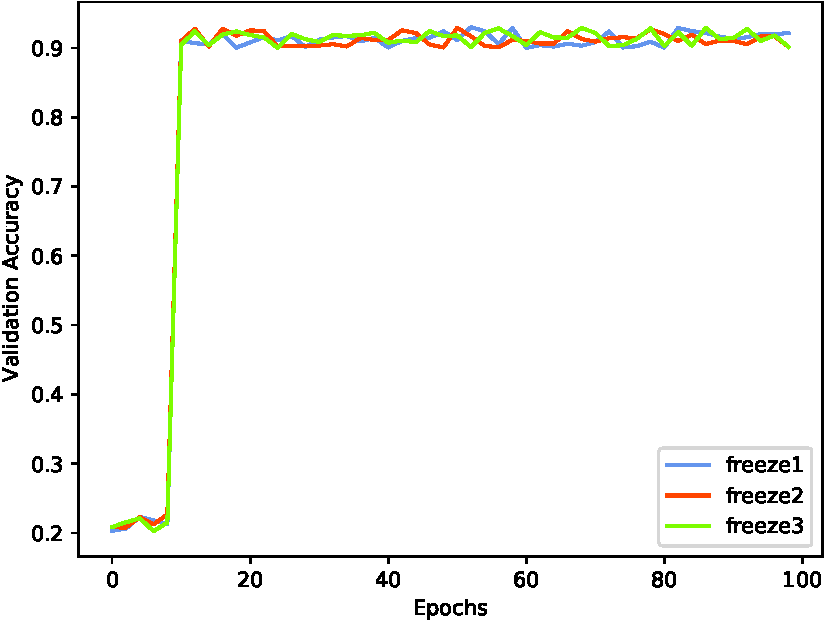
\includegraphics[
        width=0.6\textwidth,
        keepaspectratio
    ]{acc.pdf}
    \caption{Validation accuracy.}
    \label{fig:resAcc}
\end{figure*}

Although the parameters of the network 
were initialized with the model trained by 
ImageNet at the beginning of the training 
phase, and the model is far from the final 
solution, we adopt a warmup strategy by using 
a very small learning rate 0.00001 in the 
first 5 epochs and then switch to the 
initial learning rate when the training 
process is stable. Besides, for every 5 
epochs, we compare the performance between 
the current model and the best model of 
previous epochs. If the previous one 
performs better, the parameters in the 
former model will be loaded into the 
current model before the next epoch starts.

\subsection{Results}
\label{sec:ExpRes}

For mammography image recognition, the DDSM 
dataset contains 753 calcification cases, 
providing a data-set size capable of 
analyzing decision support systems in 
mammography. We also compared the results 
on the DDSM dataset with other methods 
including CNN feature-based methods. 
As shown in 
Table~\ref{tab:tabPerf},
the proposed method achieved high accuracy 
close to other methods without obvious 
advantages on the DDSM dataset. We also trained 
3 models concentrating on different kind
of features by freezing different 
parameters during training. This method 
performs better on a fine-grained 
classification task. Our method achieved 
high accuracy on this task, significantly 
higher than other methods.

\begin{table*}[!ht]
    \caption{Performance comparing to 
        different methods}
    \label{tab:tabPerf}
    \setlength{\arrayrulewidth}{1.05 pt}
    \renewcommand{\arraystretch}{1.1}
    \begin{tabular*}{1.0\textwidth}{
        @{
            \extracolsep{\fill}
        }ll
    }
        \hline
        Method & Accuracy($\%$) \\
        \hline
        SIFT-BoVW       & 89.05 \\
        VGGNet          & 90.01 \\
        AGNet           & 91.28 \\
        Inception       & 93.48 \\
        DenseNet        & 93.70 \\
        Our             & 94.68 \\
        \hline
    \end{tabular*}
\end{table*}

\subsection{Statistical analysis of fusion method}
\label{ExpSA}

In the previous sections, we have proposed 
a method which fuses 3 models with different 
layers’ parameters frozen to improve 
performance, particularly in 
Section~\ref{sec:MethNetFea} 
we mention that different models 
concentrate on different aspects of input 
images. To evaluate the diversity of 3 
models, we conduct statistical analysis with 
a series of ablation studies.

Firstly, we try to fuse any 2 models of 3 
models with different frozen parameters and 
calculate their accuracies on the test set 
comparing to a single model. Details of
the results are listed in 
Table~\ref{tab:tabFusionAny2}. 
F1–F4 represent model Freeze1 to Freeze4 
respectively and \& means fusing two
models together, for instance, F1\&F2 
means fusing model Freeze1 and Freeze2. 
According to the results, we find that 
fusing any of 2 models always performs 
better than a single one for each category. 
It can be concluded that models with 
different layers’ parameters frozen focus 
on different features of images in different 
categories, which leads to the fused network 
model get better performance.

\begin{table*}[!ht]
    \caption{Results of fusing any 2 models}
    \label{tab:tabFusionAny2}
    \setlength{\arrayrulewidth}{1.05 pt}
    \renewcommand{\arraystretch}{1.1}
    \begin{tabular*}{1.0\textwidth}{
        @{
            \extracolsep{\fill}
        }lcccccc
    }
        \hline
        
        Category & F1($\%$) & F2($\%$) & F3($\%$) 
        & F1$\&$F2($\%$) 
        & F1$\&$F3($\%$)  
        & F2$\&$F3($\%$)  \\
        
        \hline
        
        1 & 90.55 & 89.60 & 92.06 
        & 92.30 & 93.05 & 93.05 \\
        
        2 & 89.03 & 91.13 & 93.37 
        & 92.08 & 96.02 & 97.06 \\
        
        3 & 90.37 & 93.02 & 91.07 
        & 93.51 & 93.60 & 94.05 \\
        
        4 & 88.70 & 88.67 & 89.06 
        & 92.07 & 93.05 & 94.08 \\
        
        5 & 89.50 & 89.60 & 90.05 
        & 92.30 & 94.70 & 95.05 \\
        
        6 & 92.06 & 89.09 & 94.06 
        & 91.03 & 94.03 & 97.04 \\
        
        7 & 91.05 & 89.60 & 92.06 
        & 92.30 & 93.05 & 96.02 \\
        
        \hline
    \end{tabular*}
\end{table*}

In addition, when testing each single 
network’s performance, we count the numbers 
of instances that only one model recognizes 
them wrongly while the other three predict 
correctly. As shown in columns from 3 to 6 
in Table~\ref{tab:tabFusionAny1}, 3 models 
don’t give the same predicting result of
every image in each category. For each 
category, there are dozens of images which 
recognized wrongly by only one model, 
and the other 2 models can recognize them 
better.

\begin{table*}[!ht]
    \caption{Comparison of number of images 
        recognized wrongly by only one model}
    \label{tab:tabFusionAny1}
    \setlength{\arrayrulewidth}{1.05 pt}
    \renewcommand{\arraystretch}{1.1}
    \begin{tabular*}{1.0\textwidth}{
        @{
            \extracolsep{\fill}
        }lccccc
    }
        \hline
        
        Category & Total & Freeze1 & Freeze2 
        & Freeze3 & All \\
        
        \hline
        
        1 & 1172 & 58 & 44 & 31 & 0 \\
        2 & 1029 & 24 & 29 & 36 & 0 \\
        3 & 1105 & 36 & 61 & 44 & 0 \\
        4 &  859 & 48 & 41 & 56 & 0 \\
        5 &  786 & 76 & 87 & 36 & 0 \\
        6 &  907 & 15 & 29 & 41 & 0 \\
        7 &  937 & 80 & 29 & 64 & 0 \\
        
        \hline
    \end{tabular*}
\end{table*}

And It can be observed that none of the images 
are wrongly recognized by all the 3 models 
at the same time, from the last column in 
Table~\ref{tab:tabFusionAny1}. 
In other words, the 3 models pay attention 
to different aspects of the images, and each 
model has its advantage and drawback.
By integrating them and fusing their 
extracted diversified features together, 
the ensemble model learns more 
representative features.

\subsection{Analysis the hash decoder}
\label{ExpHash}

In this work, one of the innovation points, is to 
employ a hash decoder to reduce the difficulty
of computing the high dimenision parameters. A 
natural alternative to the hash decoder is
a simple fully-connected layer followed by 
a sigmoid layer of restricting the output 
values’ range in [0, 1]. To investigate the 
effectiveness of the hash decoder. Implement 
and evaluate a single deep network-based
DenseNet, connecting with its alternative
choice which is a fully network. In the end,
we employe a single classifier based SVM. To
do this, to prove our hash decoder is 
effective. As can be seen from 
Table~\ref{tab:tabHash}, 
the results of the proposed method outperform 
the competitor with the alternative. For 
example, the architecture with hash decoder 
achieves the accuracy of 0.581 with 48 bits, which 
indicates an improvement of 19.7$\%$ over the 
FC alternative. The underlying reason for
the improvement may be that, compared to the 
FC alternative, the output hash codes from 
the hash decoder are less redundant to each 
other.

\begin{table*}[!ht]
    \caption{Comparison results of the hash 
        decoder and fully connection}
    \label{tab:tabHash}
    \setlength{\arrayrulewidth}{1.05 pt}
    \renewcommand{\arraystretch}{1.1}
    \begin{tabular*}{1.0\textwidth}{
        @{
            \extracolsep{\fill}
        }lllll
    }
        \hline
        
        Method(MAP) & 12 bits & 24 bits & 32 bits & 48 bits \\
                
        \hline

        FC    & 0.877 & 0.896 & 0.909 & 0.912 \\       
        Ours  & 0.899 & 0.914 & 0.925 & 0.923 \\
        
        \hline
    \end{tabular*}
\end{table*}

\subsection{Comparing to the single classifier}
\label{ExpCls}

To investigate the effectiveness of the fusion
of the classifiers. A single DenseNet is employed
for this experiment, beacause it can maintain 
the invariance of the feature vector and enlarging 
the impact of classifier differences on test 
results. The specific 
experimental results are shown in the 
Table~\ref{tab:tabCls}. From the data in the 
table, we can see that the difference between 
different classifiers is more obvious, and 
the effect of random forest is better, but 
the result of the fused classifier is the best. 
The reason for this is that the principle of 
different classifiers is different and the 
sensitivity of features is different. It is 
obvious that the results of the fusion 
classifier can make the accuracy more reliable.

\begin{table*}[!ht]
    \caption{Comparison results of the 
        classifers}
    \label{tab:tabCls}
    \setlength{\arrayrulewidth}{1.05 pt}
    \renewcommand{\arraystretch}{1.1}
    \begin{tabular*}{1.0\textwidth}{
        @{
            \extracolsep{\fill}
        }ll
    }
        \hline
        
        Classifier & Accuracy($\%$) \\
                
        \hline

        k-NN            & 83.50 \\ 
        SVM             & 85.70 \\ 
        RandomForest    & 87.09 \\ 
        Ours            & 91.49 \\
        
        \hline
    \end{tabular*}
\end{table*}

\subsection{Comparing to single network methods}
\label{ExpCS}

There have been approaches with single 
network structures applied on DDSM,
well-performed structures like VGGNet, 
Inception, ResNet and etc are used as 
the backbones for constructing the networks 
of mammography image recognition approaches. 
To figure out which backbone is most suitable
for this task, the experiments are conducted 
to test the performance of the network with 
different backbones. 
Figure~\ref{fig:resAccDiff} shows the 
accuracy of several backbones we tried on the 
validation set during 100 training epochs. 
In the first 5 epochs, the accuracy grows 
slowly because of the warmup strategy 
mentioned in Section~\ref{sec:ExpStra}, 
and the learning rate is set to a 
relatively small value before the training 
process is stable. We found the accuracy of 
DenseNet is slightly higher than other mod-
els in the experiment. Hence it is used as 
one of the backbones.

\begin{figure*}[!ht]
    \centering
    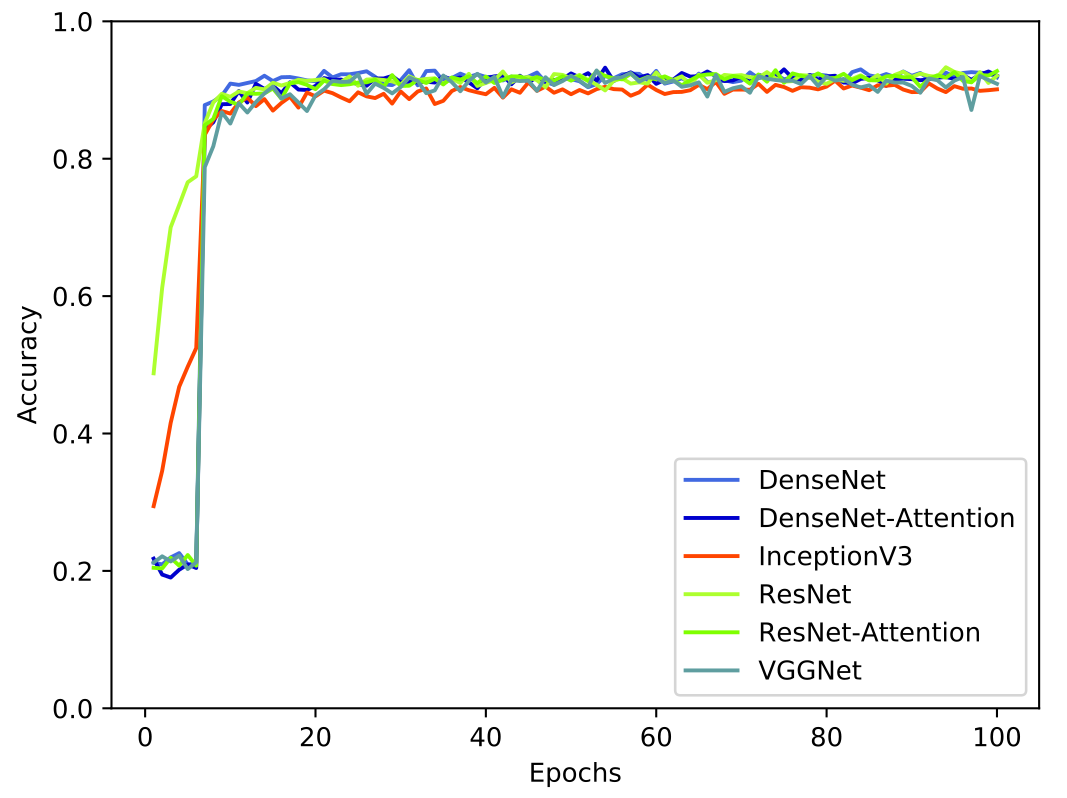
\includegraphics[
        width=0.6\textwidth,
        keepaspectratio
    ]{acc_back.png}
    \caption{Validation accuracy of different 
        backbone.}
    \label{fig:resAccDiff}
\end{figure*} 

The proposed transfer learning model 
fusion method is shown in 
Figure~\ref{fig:extrFusion}, 
3 models are trained in parallel with 
different frozen parameters. weight of each 
model is set manually according to the 
singles model’s accuracy. The accuracy of 
each single model with different frozen 
parameters is shown in 
Table~\ref{tab:tabFusionPara}. 
For instance, model Freeze1 represents the 
top row in 
Figure~\ref{fig:extrFusion}, 
which is the model with the most frozen 
parameters. In our work, 
we test different weights for each model 
according to their accuracies on the 
validation set, as shown in 
Figure~\ref{fig:resAcc}. 
Lastly, the weights 
for 3 models are set to [0.4, 0.4, 0.3].

\subsection{Comparing different network fusion 
    methods}
\label{ExpCD}

\begin{figure*}[!ht]
    \centering
    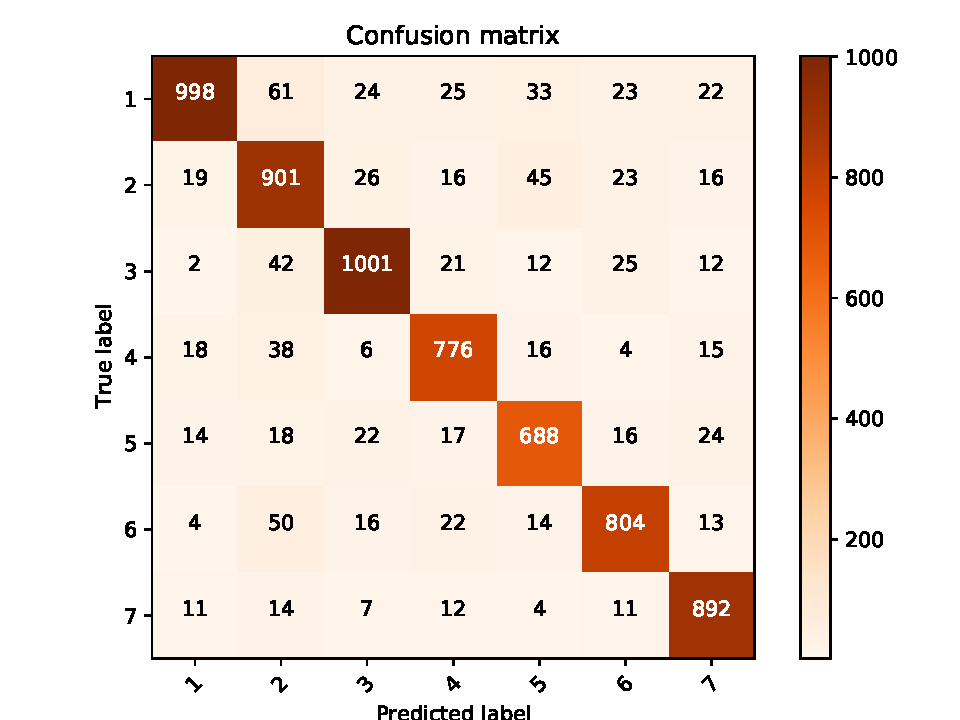
\includegraphics[
        width=0.49\textwidth,
        keepaspectratio
    ]{nonnorm_f1.pdf}
    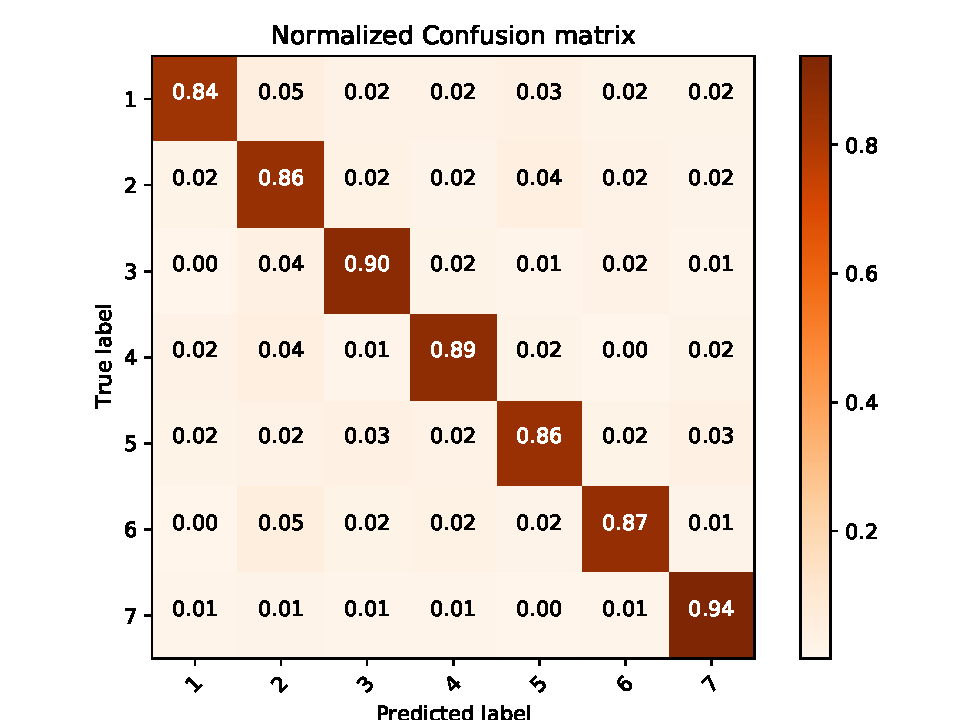
\includegraphics[
        width=0.49\textwidth,
        keepaspectratio
    ]{norm_f1.pdf}
    \caption{Confusion matrices produced by the 
        first frozen models on the test set}
    \label{fig:resFreeze1}
\end{figure*}   

\begin{figure*}[!ht]
    \centering
    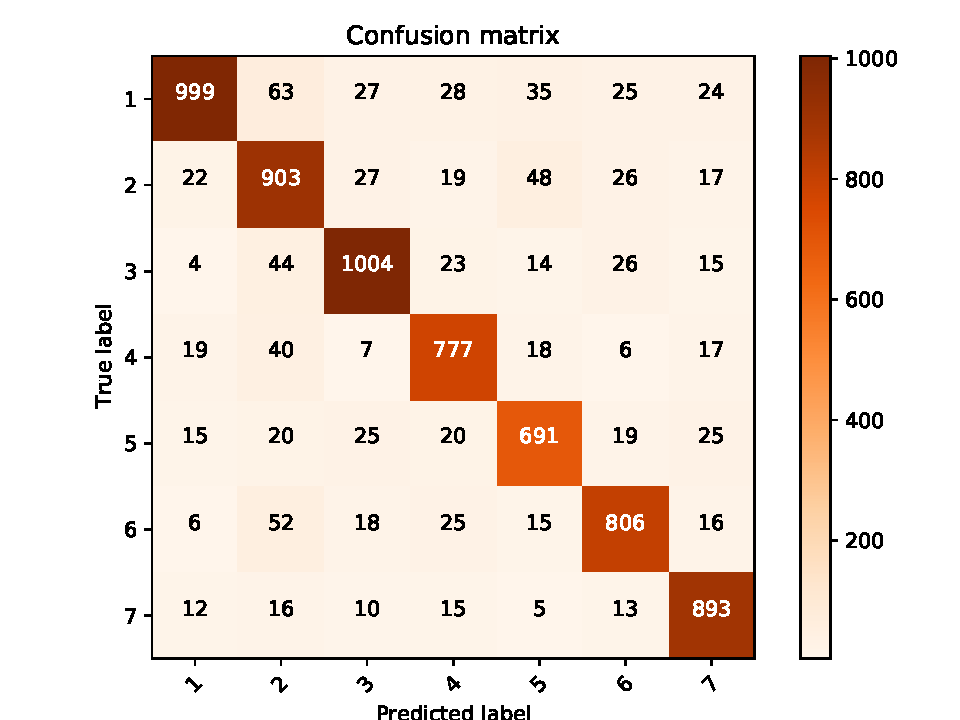
\includegraphics[
        width=0.49\textwidth,
        keepaspectratio
    ]{nonnorm_f2.pdf}
    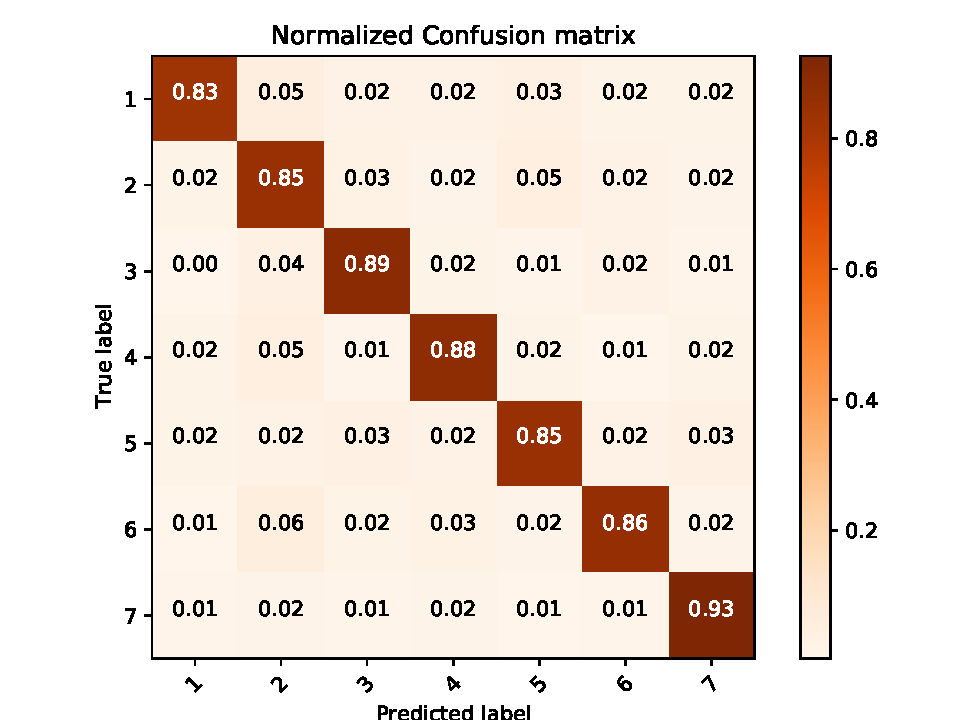
\includegraphics[
        width=0.49\textwidth,
        keepaspectratio
    ]{norm_f2.pdf}
    \caption{Confusion matrices produced by the 
        second frozen models on the test set}
    \label{fig:resFreeze2}
\end{figure*} 

\begin{figure*}[!ht]
    \centering
    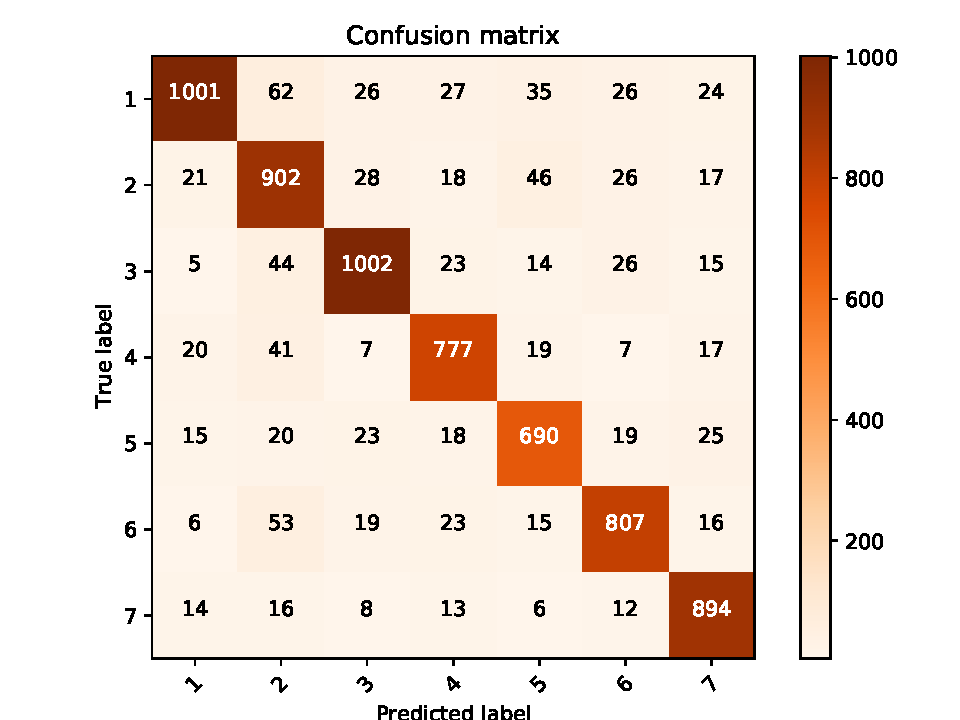
\includegraphics[
        width=0.49\textwidth,
        keepaspectratio
    ]{nonnorm_f3.pdf}
    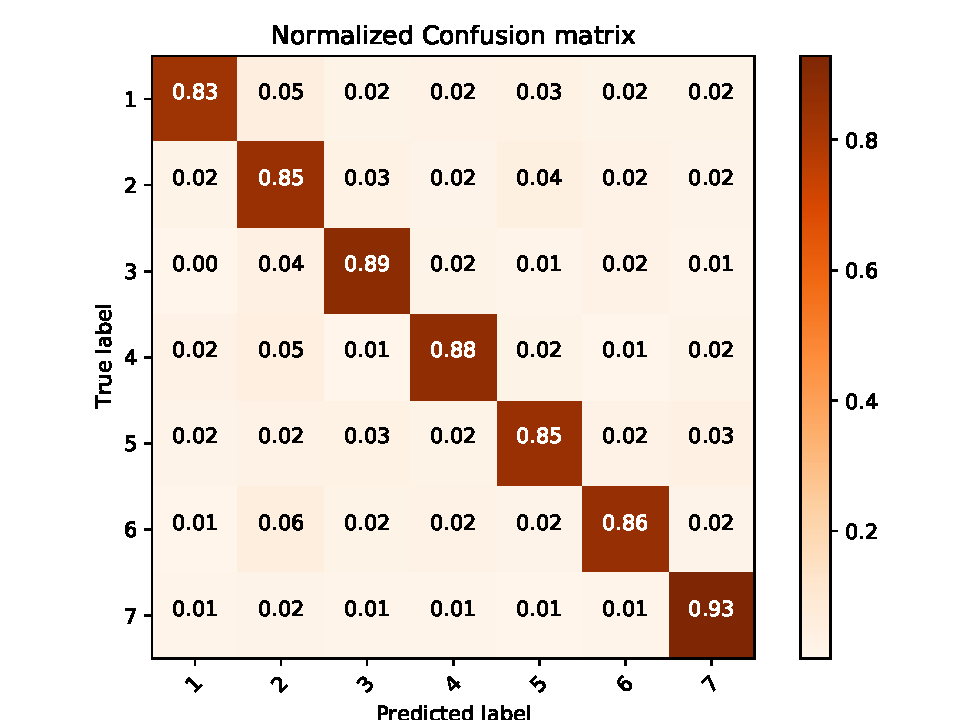
\includegraphics[
        width=0.49\textwidth,
        keepaspectratio
    ]{norm_f3.pdf}
    \caption{Confusion matrices produced by the 
        thirty frozen models on the test set}
    \label{fig:resFreeze3}
\end{figure*} 

\begin{table*}[!ht]
    \caption{Comparing with the single network 
        based methods on DDSM dataset}
    \label{tab:tabFusionNet}
    \setlength{\arrayrulewidth}{1.05 pt}
    \renewcommand{\arraystretch}{1.1}
    \begin{tabular*}{1.0\textwidth}{
        @{
            \extracolsep{\fill}
        }lll
    }
        \hline
        
        Method & Accuracy($\%$) 
        & Average inference time (ms) \\
        
        \hline
        
        VGGNet based        & 90.09 & 6.062 \\
        InceptionV3 based   & 92.16 & 2.396 \\
        ResNet50 based      & 93.08 & 3.006 \\
        DenseNet based      & 92.67 & 3.762 \\
        Our                 & 94.48 & 15.052 \\
        
        \hline
    \end{tabular*}
\end{table*}

We have proposed a method of fusing 3 models 
with different network structure but different 
frozen parameters. This idea is inspired by AGNet, 
a method enriching extracted features by combining 
2 networks with a weighted sum. Due to the 
different topological structures, the relationship
between features they extracted is relatively weak 
and we cannot assure that they have learned 
knowledge of different aspects from the training 
images.

\begin{table*}[!ht]
    \caption{Accuracies of models with different 
        parameters frozen}
    \label{tab:tabFusionPara}
    \setlength{\arrayrulewidth}{1.05 pt}
    \renewcommand{\arraystretch}{1.1}
    \begin{tabular*}{1.0\textwidth}{
        @{
            \extracolsep{\fill}
        }lll
    }
        \hline
        
        Models & Freeze params & Test accuracy($\%$) \\
        
        \hline
        
        Freeze1 & 4.76M & 93.01 \\
        Freeze2 & 3.50M & 92.36 \\
        Freeze3 & 0.95M & 91.88 \\
        Fusion  &  -    & 94.48 \\
        
        \hline
    \end{tabular*}
\end{table*}

In the experiments, we test the methods of 
fusing models in different network structures 
and on the DDSM dataset. As shown in 
Figure~\ref{fig:resFreeze1} to 
Figure~\ref{fig:resFreeze3}, 
among the 3 models we trained, Freeze3 
achieves the best result on the validation set 
during the training phase. Therefore, we try 
to fuse it with other models in different 
network structure such as VGGNet, Inception,
ResNet to check whether the fusion models 
in different network structure helps improve 
the performance or not. The parameters of 
these models are initialized by the 
corresponding pre-trained model on ImageNet 
and their shallow layers are frozen while 
training. According to the results listed in
Table~\ref{tab:tabFusionNet}, 
compared to the single network-based method, 
it has higher accuracy, but fusing 3 models 
still performs better. In this way, the 
network extracts more rich features and the 
classifier produces better recognition 
results.

\begin{figure*}[!ht]
    \centering
    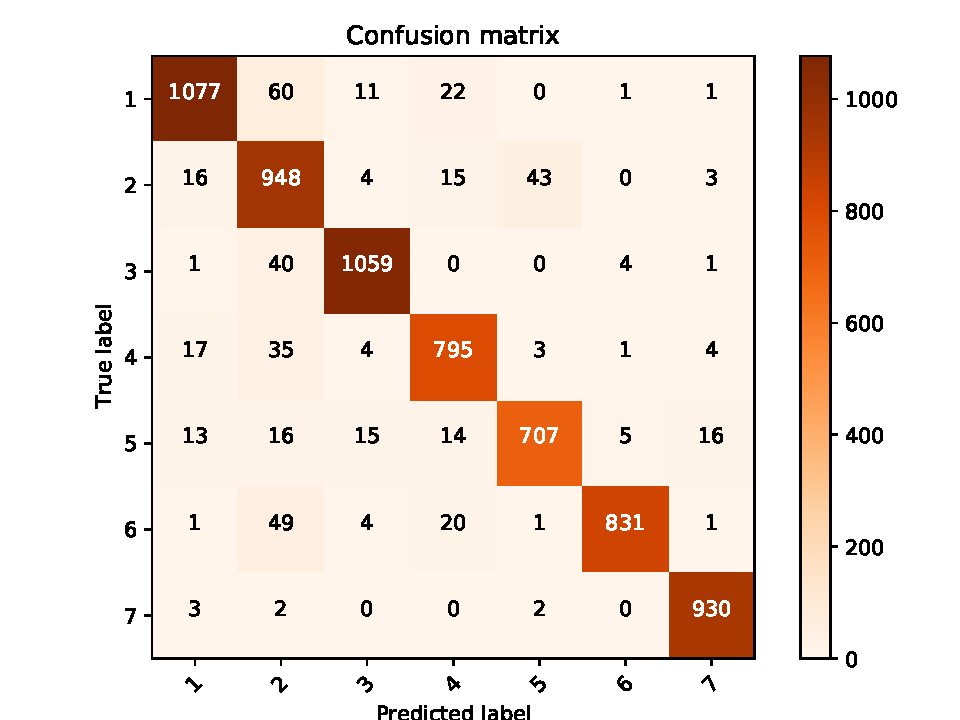
\includegraphics[
        width=0.49\textwidth,
        keepaspectratio
    ]{nonnorm.pdf}
    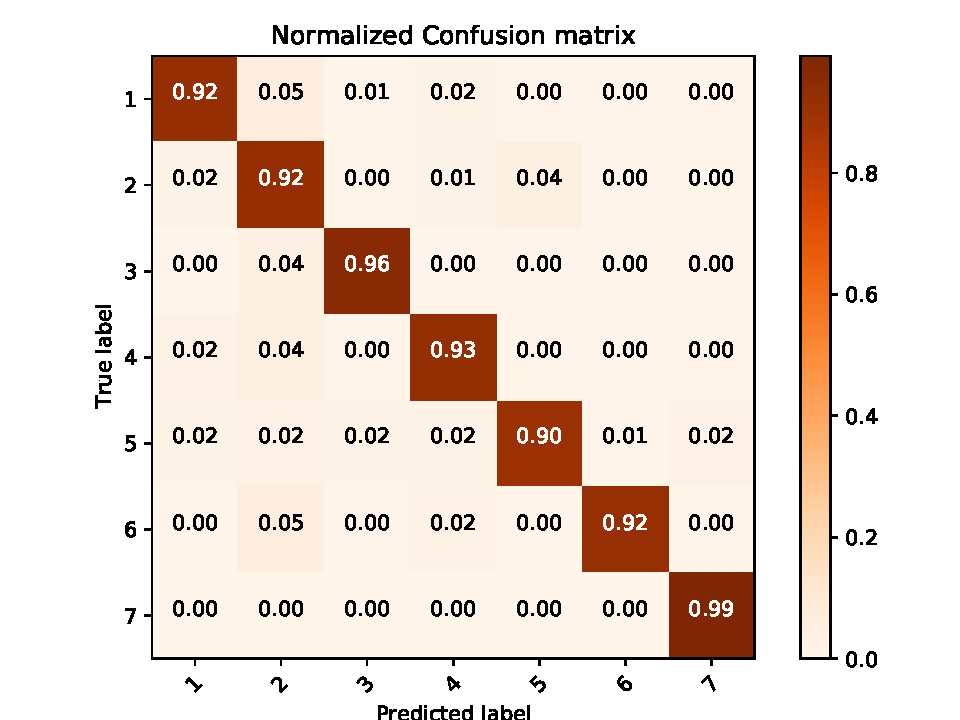
\includegraphics[
        width=0.49\textwidth,
        keepaspectratio
    ]{norm.pdf}
    \caption{Confusion matrices produced by the 
        fusion model on the test set.}
    \label{fig:resFusionMat}
\end{figure*}

Figure~\ref{fig:resFusionMat} 
shows the classification results of each 
class with confusion matrix. The accuracies 
of 7 classes are higher than 92$\%$. Because 
the features are learned from the training 
set and there are some overlapping image 
parts between classes, which contain a large 
images are more likely be wrongly classified.

\subsection{Comparing other object detection methods}
\label{ExpCD}

For the target detection module of this 
work, it is mainly based on the Faster RCNN 
framework, and the innovation of this study 
is also the innovation of the classification 
stage. For the object detection module, we 
made a simple comparison with the original 
framework model in terms of time and 
accuracy. The specific experimental results 
are shown in 
Table~\ref{tab:tabOD}. 
It is obvious from the data in the table 
that our method greatly improves the 
calculation time of the model without 
losing accuracy. Combining with our model 
framework, the reason can be clearly found 
because we have introduced a hash recoder 
module.

\begin{table*}[!ht]
    \caption{Comparing to the region RCNN}
    \label{tab:tabOD}
    \setlength{\arrayrulewidth}{1.05 pt}
    \renewcommand{\arraystretch}{1.1}
    \begin{tabular*}{1.0\textwidth}{
        @{
            \extracolsep{\fill}
        }lll
    }
        \hline
        
        Models & mAP($\%$) & time(ms) \\
        
        \hline
        
        Fast RCNN   & 60.50 & 534 \\
        Faster RCNN & 70.03 & 325 \\
        Ours        & 75.01 & 105 \\

        \hline
    \end{tabular*}
\end{table*}


\section{Conclusion}
\label{sec:Conc}

In this paper, a deep convolutional neural 
network for mammography images object detection 
task, which employing the strategy of combining 
multiple model fusion transfer and transfer 
learning to improve the classification accuracy. 
Taking advantage of multiple models’ 
representation power, the proposal achieves a 
higher accuracy than merely a single model. 
Meanwhile, the strategy applied by hash 
learning in the deep network is cited to 
enhance the generalization ability of the 
model and solve the challenge of 
high-dimensional calculation in deep learning.
In the experiments, it's found that classifying 
images based on CNN relies heavily on the 
quantity and breadth of the training data set. 
Our network is still not efficient enough to 
cover every situation of mammography diagnosed. 
In the future, we plan to collect a larger 
data set with more detailed labels and build 
a more effective architecture to further 
improve the performance of the mammography 
image object detection.

\section{Acknowledgements}
\label{sec:Acknowledgement}

This work is supported by the National 
Key R\&D Plan under Grant No. 
2018YFC1200200 and 2018YFC1200205; 
Shanghai Science and Technology Project 
in 2020 under Grant No. 20040501500.

%% bibliography
\phantomsection
\addcontentsline{toc}{section}{References}
\section*{References}
\bibliographystyle{elsarticle-harv}
\bibliography{paper}

\end{document}
